\documentclass{bredelebeamer}

%%%%%%%%%%%%%%%%%%%%%%%%%%%%%%%%%%%%%%%%%%%%%%%%
\title[Ingéniere dirigée par les Modéles]{IDM - Soutenance 1}
% Titre du diaporama

\subtitle{Groupe 1 - Les roboticiens}
% Sous-titre optionnel

\author{N. Salleron Y. Ghigoff K. Vu-Saintonge A. Archambault}
% La commande \inst{...} Permet d'afficher l' affiliation de l'intervenant.
% Si il y a plusieurs intervenants: Marcel Dupont\inst{1}, Roger Durand\inst{2}
% Il suffit alors d'ajouter un autre institut sur le modéle ci-dessous.

\date{14 Décembre 2017}
% Optionnel. La date, généralement celle du jour de la conférence

\subject{IDM}
% C'est utilisé dans les métadonnes du PDF

\logo{
%
\includegraphics[scale=0.15]{images/logo.png}
}

%%%%%%%%%%%%%%%%%%%%%%%%%%%%%%%%%%%%%%%%%%%%%%%%%%%%%%%%%%%%%%%%%%%%%
\begin{document}

\begin{frame}
  \titlepage
\end{frame}

\begin{frame}{Sommaire}
  \tableofcontents
  % possibilité d'ajouter l'option [pausesections]
\end{frame}

\section{Introduction}

\begin{frame}{Introduction}
%Texte normal \alert{Texte Alert}  \exemple{Texte exemple} \emph{Texte emphase}
\begin{columns}
\begin{column}{0.5\textwidth}
\begin{block}{Une utilisation de plus en plus populaire}
\begin{itemize}
\item Utilisation dans le cadre militaire dans les année 1990.
\item De plus en plus populaire au sein du grand public.
\item Las Vegas, CES 2016, présentation du "drone dance" par la société Parrot
\item La télévision avec "La France a un incroyable talent"
\end{itemize}
\end{block}
\end{column}
\begin{column}{0.5\textwidth}
\begin{figure}
\centering
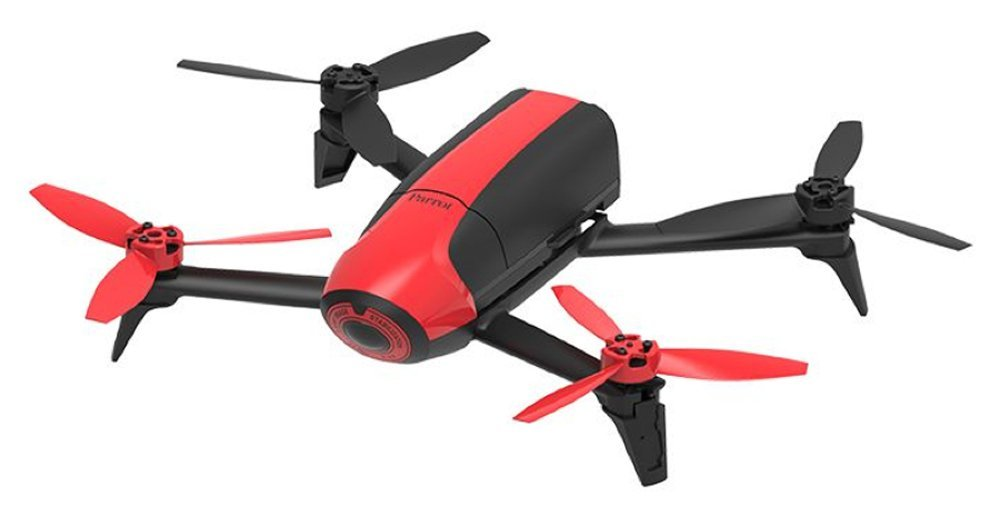
\includegraphics[scale=0.15]{images/img1.jpg}
\caption{Exemple de drone}
\end{figure}
\end{column}
\end{columns}
\end{frame}

\begin{frame}{Introduction}
%Texte normal \alert{Texte Alert}  \exemple{Texte exemple} \emph{Texte emphase}
\begin{columns}
\begin{column}{0.5\textwidth}
\begin{block}{Contexte}
\begin{itemize}
\item Domaine de la danse.
\item Préparation d'une chorégraphie et exécution sur le terrain.
\item Création d'un langage de programmation spécifique.
\end{itemize}
\end{block}
\begin{block}{Objectif}
\begin{itemize}
\item Produire un langage de programmation \alert{simple} et \alert{compréhensible} pour l'utilisateur.
\item Rendre l'utilisateur autonome.
\item Adaptable à plusieurs drones.
\item Faire danser le drone.
\end{itemize}
\end{block}
\end{column}
\begin{column}{0.5\textwidth}
\begin{figure}
\centering
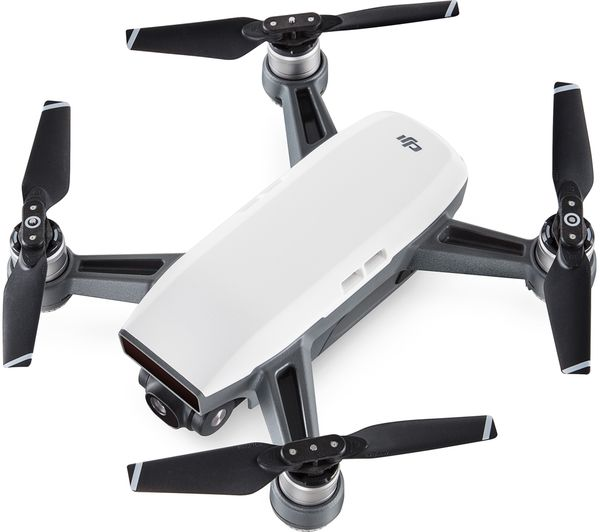
\includegraphics[scale=0.15]{images/img2.jpg}
\caption{Autre exemple de drone}
\end{figure}
\end{column}
\end{columns}
\end{frame}

\section{Editeur de langage}

\begin{frame}{Editeur de langage}
\begin{columns}
\begin{column}{0.5\textwidth}
\begin{block}{Description de l'éditeur}
Notre éditeur posséde les fonctionnalités suivantes :
\begin{itemize}
\item Auto-complétion du langage. 
\item Détection des fautes syntaxiques.
\item Détection des erreurs de cohérence dans les scénarios.
\end{itemize}
\end{block}\pause


\begin{block}{Écriture de la chorégraphie}
\begin{itemize}
\item L'utilisateur écrit sa chorégraphie par une suite d'action séparée par un retour à la ligne.
\item Une chorégraphie commence par un décollage et un atterrissage.
\item Usage possible de fonctions et d'instruction simple.
\end{itemize}
\end{block}\pause
\end{column}
\begin{column}{0.5\textwidth}
\begin{alertblock}{Conditions de fonctionnement}
\begin{itemize}
\item Le drone utilisé est un drone à hélices. 
\item Le drone est allumé, connecté via Wi-Fi à l’ordinateur.
\item Le drone doit être utilisé dans un endroit sans un vent fort.
\item Le programme utilisateur réalisé sous Eclipse Oxygen version 4.7.0.
\item Java version 1.8. 
\end{itemize}
\end{alertblock}
\vspace{80px}
\end{column}
\end{columns}
\end{frame}



\section{Fonctionnement du drone}

\begin{frame}{Fonctionnement du drone}

\begin{columns}

\begin{column}{0.65\textwidth}

\begin{block}{Mouvements sur les axes}
Le drone évoluant dans un environnement 3D, ce dernier peut effectuer différentes actions: \\
\begin{itemize}
\item Altitude : évolution sur l'axe Z. \\Correspond aux instructions "\alert{monter}" et "\alert{descendre}"
\item Roll : évolution sur l'axe X. \\Correspond aux instructions "\alert{gauche}" et "\alert{droite}"
\item Pitch: évolution sur l'axe Y. \\Correspond aux instructions "\alert{avancer}" et "\alert{reculer}"
\end{itemize}
\end{block}\pause

\begin{exampleblock}{Éléments particuliers}
\begin{itemize}
\item Décollage et Attérrissage : correspond aux instructions "\alert{decoller}" et "\alert{atterrir}"
\item Pause : correspond à l'instruction "\alert{pause}"
\item Rotation : correspond aux instructions "\alert{rotationGauche}" et "\alert{rotationDroite}"
\end{itemize}
\end{exampleblock}\pause

\end{column}
\begin{column}{0.35\textwidth}
\begin{alertblock}{Cas de la caméra}
\begin{itemize}
\item Caméra : Il n’est pas standard qu’un drone posséde une caméra.
\end{itemize}
\end{alertblock}
\begin{figure}
\centering
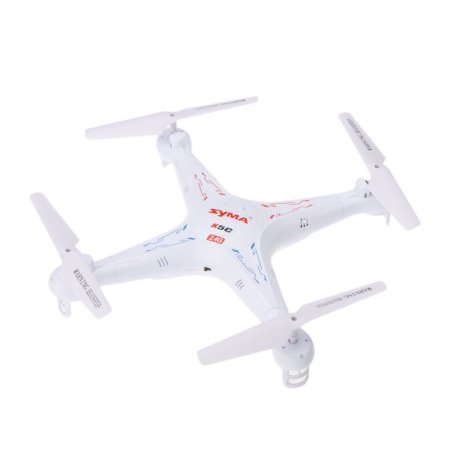
\includegraphics[scale=0.20]{images/img3.jpeg}
\caption{Exemple de drone sans caméra}
\end{figure}
\vspace{15px}
\end{column}
\end{columns}
\end{frame}

\section{Les commandes du DSL}
	\subsection{Prologue}

\begin{frame}[fragile]{Prologue}
\begin{block}{Définir 5 constantes de vol}
\begin{itemize}
\item \alert{define} \emph{vitesse\_hauteur\_max}: vitesse maximale d’élévation du drone pour la chorégraphie.
\item \alert{define} \emph{vitesse\_deplacement\_max}: vitesse maximale de déplacement sur le plan horizontal du drone pour la chorégraphie. 
\item \alert{define} \emph{vitesse\_rotation\_max}: vitesse maximale de rotation du drone pour la chorégraphie.
\item \alert{define} \emph{hauteur\_max}: Cette constante permet de limiter l’altitude maximale du drone en vol.
\item \alert{define} \emph{eloignement\_max}: Cette constante permet de contr\^oler la distance horizontale du drone en vol par rapport au point de décollage.
\end{itemize}
\end{block}


Exemple de define : 
\begin{center}
\color{Framarouge}
	define vitesse\_hauteur\_max \color{Framagris}50\%
\end{center}
\end{frame} 

	\subsection{Instructions basique} 
\begin{frame}{Instructions basique} 
Le but est de rendre accessible le pilotage de drone aux chorégraphes. 
\begin{block}{Les 11 instructions basiques}
\begin{itemize}
\item \alert{decoller}
\item \alert{atterrir}
\item \alert{pause(durée : Seconde)}
\item \alert{monter(durée : Seconde, vitesse\_verticale : Pourcentage)}
\item \alert{decendre(durée : Seconde, vitesse\_verticale : Pourcentage)}
\item \alert{avancer(durée : Seconde, vitesse\_deplacement : Pourcentage)}
\item \alert{reculer(durée : Seconde, vitesse\_deplacement : Pourcentage)}
\item \alert{gauche(durée : Seconde, vitesse\_deplacement : Pourcentage)}
\item \alert{droite(durée : Seconde, vitesse\_deplacement : Pourcentage)}
\item \alert{rotationGauche(durée : Seconde, vitesse\_rotation : Pourcentage)}
\item \alert{rotationDroite(durée : Seconde, vitesse\_rotation : Pourcentage)}
\end{itemize}
\end{block}
\begin{itemize}
\item 1er paramètre est la durée du mouvement, en Seconde.
\item 2éme paramètre est la vitesse du mouvement, en pourcentage. Il représente la vitesse du drone par rapport à la vitesse définie dans la section "prologue".
\end{itemize}
\end{frame}

	\subsection{Instructions paralléles} 
\begin{frame}{Les Instructions paralléles} 
\begin{itemize}
\item Notre langage intègre un mécanisme d'exécution d'instructions parallèle.
\item Il est possible d'ordonner au drone de faire plusieurs instructions en même temps. 
\item Mécanisme implémenter par le symbole '\&'. \pause
\item Disponible que pour certaines instructions comme :  
	\begin{enumerate}
		\item monter
		\item descendre
		\item avancer
		\item reculer
		\item gauche
		\item droite
		\item rotationGauche
		\item rotationDroite
	\end{enumerate}	\pause
\item Maximum de 3 instructions parallélisable.
\end{itemize}
\begin{tabbing}
Exemple : \=\\
	\>\color{Framarouge}monter(\color{black}1\color{Framarouge},\color{Framagris}10\%\color{Framarouge}) \& 
	\color{Framarouge}descendre(\color{black}4\color{Framarouge},\color{Framagris}20\%\color{Framarouge})\\ \pause
	\color{black}\>-> Impossible les deux commandes s'opposent.\\
	\>\color{Framarouge}gauche(\color{black}3\color{Framarouge},\color{Framagris}25\%\color{Framarouge}) \& 
	\color{Framarouge}gauche(\color{black}4\color{Framarouge},\color{Framagris}20\%\color{Framarouge})\\ \pause
	\color{black}\>-> Impossible les deux commandes sont de même type.\\
	\>\color{Framarouge}rotationDroite(\color{black}2\color{Framarouge},\color{Framagris}25\%\color{Framarouge}) \& 
	\color{Framarouge}avancer(\color{black}5\color{Framarouge},\color{Framagris}20\%\color{Framarouge})\\ \pause
	\color{black}\>-> Ok
\end{tabbing}
\end{frame}
	
	\subsection{Fonction} 
\begin{frame}{Les fonctions} 
\begin{itemize}
\item Le langage permet de définir des fonctions.
\item Les fonctions sont une suite d'instructions séquentielles.
\item Il n'est pas possible de paralléliser deux fonctions.
\item Une fonction ne peut pas s'appeler elle-même.
\item Une fonction ne peut pas appeler d'autres fonctions.
\end{itemize}


\begin{tabbing}
Exemple : \=\\
	\>\color{Framarouge}func \=\color{black}maFonction\color{Framarouge}() \{\\ 
	\>\>\color{Framarouge}rotationDroite(\color{black}2\color{Framarouge},\color{Framagris}25\%\color{Framarouge}) \& 
	\color{Framarouge}avancer(\color{black}5\color{Framarouge},\color{Framagris}20\%\color{Framarouge})\\ 
	\>\>\color{Framarouge}droite(\color{black}3\color{Framarouge},\color{Framagris}80\%\color{Framarouge})\\ 
	\>\>\color{Framarouge}avancer(\color{black}4\color{Framarouge},\color{Framagris}10\%\color{Framarouge})\\ 
	\>\color{Framarouge}\}
\end{tabbing}
	
	
	
	
\end{frame}


\subsection{Le bloc "main" et les bibliothéques de fonctions} 
\begin{frame}{Le bloc "main" et les bibliothéques de fonctions} 

\begin{columns}

\begin{column}{0.5\textwidth}


Le point d'entrée "main \{ \}" :\\
\begin{itemize}
\item Défini par le mot clé "main"
\item Le contenu de ce bloc d'instruction sera exécuté.
\item Il est le seul à pouvoir appeler des fonctions.
\end{itemize}\pause

\begin{tabbing}
Exemple : \=\\
	\>\color{Framarouge}main  \{\=\\ 
	\>\>\color{Framarouge}decoller()\\
	\>\>\color{Framarouge}gauche(\color{black}1\color{Framarouge},\color{Framagris}10\%\color{Framarouge})\\ 
	\>\>\color{Framarouge}avancer(\color{black}4\color{Framarouge},\color{Framagris}34\%\color{Framarouge})\\
	\>\>\color{Framarouge}maFonction()\\ 
	\>\>\color{Framarouge}atterrir()\\
	\>\color{Framarouge}\}\\
	
	\>\color{Framarouge}func \=\color{black}maFonction\color{Framarouge}() \{\\ 
	\>\>\color{Framarouge}rotationDroite(\color{black}2\color{Framarouge},\color{Framagris}25\%\color{Framarouge}) \& 
	\color{Framarouge}avancer(\color{black}5\color{Framarouge},\color{Framagris}20\%\color{Framarouge})\\ 
	\>\>\color{Framarouge}droite(\color{black}3\color{Framarouge},\color{Framagris}80\%\color{Framarouge})\\ 
	\>\>\color{Framarouge}avancer(\color{black}4\color{Framarouge},\color{Framagris}10\%\color{Framarouge})\\ 
	\>\color{Framarouge}\}\pause

\end{tabbing}	
\end{column}
\begin{column}{0.5\textwidth}
Les bibliothéques de fonctions:\\
\begin{itemize}
\item Possibilité d'utiliser des fonctions définies dans des fichiers .drone.
\item Doivent être dans le même répertoire que le fichier appelant les fonctions.
\end{itemize}\pause
\begin{tabbing}
Exemple :\=\\
            \>\color{Framarouge}import <\color{black}monFichier.drone\color{Framarouge}>
\end{tabbing}		
\vspace{90px}
\end{column}
\end{columns}

\end{frame}

\section{Tests de validations}

\begin{frame}{Tests de validations} 
\begin{tabular}{|p{0.25\linewidth} | p{0.70\linewidth}|}
\rowcolor[RGB]{18,144,176}\color{white}Validation :& \color{white}TVEDT-01\\
\hline
Contexte :& L'utilisateur a démarré son éditeur.\\
\hline
Entrée :& aucune \\
\hline
Scénario :&  \begin{minipage}[t]{0.7\textwidth}
    \vspace{1px}
   
    \color{Framarouge}define vitesse\_hauteur\_max \color{Framagris}100\%
    \\\color{Framarouge}define vitesse\_deplacement\_max  \color{Framagris}40\%
    \\\color{Framarouge}define vitesse\_rotation\_max  \color{Framagris}50\%
    \\\color{Framarouge}define hauteur\_max  \color{black}10
    \\\color{Framarouge}define eloignement\_max \color{black}4\\
    \begin{tabbing}
    
	\color{Framarouge}main  \{\=\\ 
	\>\color{Framarouge}decoller()\\
	\>\color{Framarouge}gauche(\color{black}1\color{Framarouge},\color{Framagris}10\%\color{Framarouge})\\ 
	\>\color{Framarouge}atterrir()\\
	\color{Framarouge}\}\\
    
    \end{tabbing}

    
\end{minipage} \\
\hline
Résultat attendu:& Aucune erreur n'est détectée par l'éditeur. \\
\hline
\end{tabular}

\end{frame}

\begin{frame}{Tests de validations} 
\begin{tabular}{|p{0.25\linewidth} | p{0.70\linewidth}|}
\rowcolor[RGB]{18,144,176}\color{white}Validation :& \color{white}TVEDT-02\\
\hline
Contexte :& L'utilisateur a démarré son éditeur.\\
\hline
Entrée :& aucune \\
\hline
Scénario :&  \begin{minipage}[t]{0.7\textwidth}
    \vspace{1px}
   
    \color{Framarouge}define vitesse\_hauteur\_max \color{Framagris}100\%
    \\\color{Framarouge}define vitesse\_deplacement\_max  \color{Framagris}40\%
    \\\color{Framarouge}define vitesse\_rotation\_max  \color{Framagris}50\%
    \\\color{Framarouge}define hauteur\_max  \color{black}10
    \\\color{Framarouge}define eloignement\_max \color{black}4\\
    \begin{tabbing}
    
	\color{Framarouge}main  \{\=\\ 
	\>\color{Framarouge}decoller()\\
	\>\color{Framarouge}monter(\color{black}1\color{Framarouge},\color{Framagris}20\%\color{Framarouge})\\ 
	\>\color{Framarouge}avancer(\color{black}1\color{Framarouge},\color{Framagris}20\%\color{Framarouge})\\ 
	\>\color{Framarouge}reculer(\color{black}1\color{Framarouge},\color{Framagris}20\%\color{Framarouge})\\ 
	\>\color{Framarouge}atterrir()\\
	\color{Framarouge}\}\\
    
    \end{tabbing}
\end{minipage} \\
\hline
Résultat attendu:& Aucune erreur n'est détectée par l'éditeur. \\
\hline
\end{tabular}

\end{frame}



\begin{frame}{Tests de validations} 
\begin{tabular}{|p{0.25\linewidth} | p{0.70\linewidth}|}
\rowcolor[RGB]{18,144,176}\color{white}Validation :& \color{white}TVEDT-03\\
\hline
Contexte :& L'utilisateur a démarré son éditeur.\\
\hline
Entrée :& aucune \\
\hline
Scénario :&  \begin{minipage}[t]{0.7\textwidth}
    \vspace{1px}
   
    \color{Framarouge}define vitesse\_hauteur\_max \color{Framagris}100\%
    \\\color{Framarouge}define vitesse\_deplacement\_max  \color{Framagris}40\%
    \\\color{Framarouge}define vitesse\_rotation\_max  \color{Framagris}50\%
    \\\color{Framarouge}define hauteur\_max  \color{black}10
    \\\color{Framarouge}define eloignement\_max \color{black}4\\
    \begin{tabbing}
    
	\color{Framarouge}main  \{\=\\ 
	\>\color{Framarouge}decoller()\\
	\>\color{Framarouge}blablabla()\\ 
	\>\color{Framarouge}atterrir()\\
	\color{Framarouge}\}\\
    
    \end{tabbing}
\end{minipage} \\
\hline
Résultat attendu:& Une erreur est détectée sur la commande \textit{blabalbla}.  \\
\hline
\end{tabular}

\end{frame}


\begin{frame}{Tests de validations} 
\begin{tabular}{|p{0.25\linewidth} | p{0.70\linewidth}|}
\rowcolor[RGB]{18,144,176}\color{white}Validation :& \color{white}TVEDT-04\\
\hline
Contexte :& L'utilisateur a démarré son éditeur.\\
\hline
Entrée :& aucune \\
\hline
Scénario :&  \begin{minipage}[t]{0.7\textwidth}
    \vspace{1px}
   
    \color{Framarouge}define vitesse\_hauteur\_max \color{Framagris}100\%
    \\\color{Framarouge}define vitesse\_deplacement\_max  \color{Framagris}40\%
    \\\color{Framarouge}define vitesse\_rotation\_max  \color{Framagris}50\%
    \\\color{Framarouge}define hauteur\_max  \color{black}10
    \\\color{Framarouge}define eloignement\_max \color{black}4\\
    \begin{tabbing}
    
	\color{Framarouge}main  \{\=\\ 
	\>\color{Framarouge}decoller()\\
	\>\color{Framarouge}monter(\color{black}"hello"\color{Framarouge})\\ 
	\>\color{Framarouge}atterrir()\\
	\color{Framarouge}\}\\
    
    \end{tabbing}
\end{minipage} \\
\hline
Résultat attendu:& Une erreur est détectée sur la commande \textit{monter}. \\
\hline
\end{tabular}

\end{frame}


\begin{frame}{Tests de validations} 
\begin{tabular}{|p{0.25\linewidth} | p{0.70\linewidth}|}
\rowcolor[RGB]{18,144,176}\color{white}Validation :& \color{white}TVEDT-05\\
\hline
Contexte :& L'utilisateur a démarré son éditeur.\\
\hline
Entrée :& aucune \\
\hline
Scénario :&  \begin{minipage}[t]{0.7\textwidth}
    \vspace{1px}
   
    \color{Framarouge}define vitesse\_hauteur\_max \color{Framagris}100\%
    \\\color{Framarouge}define vitesse\_deplacement\_max  \color{Framagris}40\%
    \\\color{Framarouge}define vitesse\_rotation\_max  \color{Framagris}50\%
    \\\color{Framarouge}define hauteur\_max  \color{black}10
    \\\color{Framarouge}define eloignement\_max \color{black}4\\
    \begin{tabbing}
    
	\color{Framarouge}main  \{\=\\ 
	\>\color{Framarouge}decoller()\\
	\>\color{Framarouge}atterrir()\\
	\>\color{Framarouge}monter(\color{black}1\color{Framarouge},\color{Framagris}20\%\color{Framarouge})\\ 
	\color{Framarouge}\}\\
    
    \end{tabbing}
\end{minipage} \\
\hline
Résultat attendu:& Une erreur est détectée sur la commande \textit{monter}. \\
\hline
\end{tabular}

\end{frame}


\begin{frame}{Tests de validations} 
\begin{tabular}{|p{0.25\linewidth} | p{0.70\linewidth}|}
\rowcolor[RGB]{18,144,176}\color{white}Validation :& \color{white}TVEDT-06\\
\hline
Contexte :& L'utilisateur a démarré son éditeur.\\
\hline
Entrée :& aucune \\
\hline
Scénario :&  \begin{minipage}[t]{0.7\textwidth}
    \vspace{1px}
   
    \color{Framarouge}define vitesse\_hauteur\_max \color{Framagris}100\%
    \\\color{Framarouge}define vitesse\_deplacement\_max  \color{Framagris}40\%
    \\\color{Framarouge}define vitesse\_rotation\_max  \color{Framagris}50\%
    \\\color{Framarouge}define hauteur\_max  \color{black}10
    \\\color{Framarouge}define eloignement\_max \color{black}4\\
    \begin{tabbing}
    
	\color{Framarouge}main  \{\=\\ 
	\>\color{Framarouge}monter(\color{black}1\color{Framarouge},\color{Framagris}20\%\color{Framarouge})\\ 
	\>\color{Framarouge}decoller()\\
	\>\color{Framarouge}atterrir()\\
	\color{Framarouge}\}\\
    
    \end{tabbing}
\end{minipage} \\
\hline
Résultat attendu:& Une erreur est détectée sur la commande \textit{monter}.\\
\hline
\end{tabular}

\end{frame}


\begin{frame}{Tests de validations} 
\begin{tabular}{|p{0.25\linewidth} | p{0.70\linewidth}|}
\rowcolor[RGB]{18,144,176}\color{white}Validation :& \color{white}TVEDT-07\\
\hline
Contexte :& L'utilisateur a démarré son éditeur.\\
\hline
Entrée :& aucune \\
\hline
Scénario :&  \begin{minipage}[t]{0.7\textwidth}
    \vspace{1px}
   
    \color{Framarouge}define vitesse\_hauteur\_max \color{Framagris}100\%
    \\\color{Framarouge}define vitesse\_deplacement\_max  \color{Framagris}40\%
    \\\color{Framarouge}define vitesse\_rotation\_max  \color{Framagris}50\%
    \\\color{Framarouge}define hauteur\_max  \color{black}10
    \\\color{Framarouge}define eloignement\_max \color{black}4\\
    \begin{tabbing}
    
	\color{Framarouge}main  \{\=\\ 
	\>\color{Framarouge}decoller()\\
	\>\color{Framarouge}decoller()\\
	\>\color{Framarouge}atterrir()\\
	\color{Framarouge}\}\\
    
    \end{tabbing}
\end{minipage} \\
\hline
Résultat attendu:& Une erreur est détectée sur la deuxième commande \textit{decoller}.\\
\hline
\end{tabular}

\end{frame}

\begin{frame}{Tests de validations} 
\begin{tabular}{|p{0.25\linewidth} | p{0.70\linewidth}|}
\rowcolor[RGB]{18,144,176}\color{white}Validation :& \color{white}TVEDT-08\\
\hline
Contexte :& L'utilisateur a démarré son éditeur.\\
\hline
Entrée :& aucune \\
\hline
Scénario :&  \begin{minipage}[t]{0.7\textwidth}
    \vspace{1px}
   
    \color{Framarouge}define vitesse\_hauteur\_max \color{Framagris}100\%
    \\\color{Framarouge}define vitesse\_deplacement\_max  \color{Framagris}40\%
    \\\color{Framarouge}define vitesse\_rotation\_max  \color{Framagris}50\%
    \\\color{Framarouge}define hauteur\_max  \color{black}10
    \\\color{Framarouge}define eloignement\_max \color{black}4\\
    \begin{tabbing}
    
	\color{Framarouge}main  \{\=\\ 
	\>\color{Framarouge}decoller()\\
	\>\color{Framarouge}atterrir()\\
	\>\color{Framarouge}atterrir()\\
	\color{Framarouge}\}\\
    
    \end{tabbing}
\end{minipage} \\
\hline
Résultat attendu:& Une erreur est détectée sur la deuxième commande \textit{atterrir}.\\
\hline
\end{tabular}

\end{frame}



\begin{frame}{Tests de validations} 
\begin{tabular}{|p{0.25\linewidth} | p{0.70\linewidth}|}
\rowcolor[RGB]{18,144,176}\color{white}Validation :& \color{white}TVEDT-09\\
\hline
Contexte :& L'utilisateur a démarré son éditeur.\\
\hline
Entrée :& aucune \\
\hline
Scénario :&  \begin{minipage}[t]{0.7\textwidth}
    \vspace{1px}
   
    \color{Framarouge}define vitesse\_hauteur\_max \color{Framagris}100\%
    \\\color{Framarouge}define vitesse\_deplacement\_max  \color{Framagris}40\%
    \\\color{Framarouge}define vitesse\_rotation\_max  \color{Framagris}50\%
    \\\color{Framarouge}define hauteur\_max  \color{black}10
    \\\color{Framarouge}define eloignement\_max \color{black}4\\
    \begin{tabbing}
    
	\color{Framarouge}main  \{\=\\ 
	\>\color{Framarouge}decoller()\\
	\>\color{Framarouge}aller\_retour()\\
	\>\color{Framarouge}atterrir()\\
	\color{Framarouge}\}\\
    
    \color{Framarouge}func \=\color{black}aller\_retour\color{Framarouge}() \{\\ 
	\>\color{Framarouge}avancer(\color{black}5\color{Framarouge},\color{Framagris}20\%\color{Framarouge})\\ 
	\>\color{Framarouge}reculer(\color{black}5\color{Framarouge},\color{Framagris}20\%\color{Framarouge})\\ 
	\color{Framarouge}\}
    \end{tabbing}
\end{minipage} \\
\hline
Résultat attendu:& Aucune erreur n'est détectée par l'éditeur.\\
\hline
\end{tabular}

\end{frame}


\begin{frame}{Tests de validations} 
\begin{tabular}{|p{0.25\linewidth} | p{0.70\linewidth}|}
\rowcolor[RGB]{18,144,176}\color{white}Validation :& \color{white}TVEDT-10\\
\hline
Contexte :& L'utilisateur a démarré son éditeur.\\
\hline
Entrée :& aucune \\
\hline
Scénario :&  \begin{minipage}[t]{0.7\textwidth}
    \vspace{1px}
   
    \color{Framarouge}define vitesse\_hauteur\_max \color{Framagris}100\%
    \\\color{Framarouge}define vitesse\_deplacement\_max  \color{Framagris}40\%
    \\\color{Framarouge}define vitesse\_rotation\_max  \color{Framagris}50\%
    \\\color{Framarouge}define hauteur\_max  \color{black}10
    \\\color{Framarouge}define eloignement\_max \color{black}4\\
    \begin{tabbing}
    
	\color{Framarouge}main  \{\=\\ 
	\>\color{Framarouge}decoller()\\
	\>\color{Framarouge}foo()\\
	\>\color{Framarouge}atterrir()\\
	\color{Framarouge}\}\\
    
    \color{Framarouge}func \=\color{black}bar\color{Framarouge}() \{\\ 
	\>\color{Framarouge}avancer(\color{black}5\color{Framarouge},\color{Framagris}20\%\color{Framarouge})\\ 
	\color{Framarouge}\}
    \end{tabbing}
\end{minipage} \\
\hline
Résultat attendu:& Une erreur est détectée sur l'appel de la fonction \textit{foo}.\\
\hline
\end{tabular}

\end{frame}


\begin{frame}{Tests de validations} 
\begin{tabular}{|p{0.25\linewidth} | p{0.70\linewidth}|}
\rowcolor[RGB]{18,144,176}\color{white}Validation :& \color{white}TVEDT-11\\
\hline
Contexte :& L'utilisateur a démarré son éditeur.\\
\hline
Entrée :& aucune \\
\hline
Scénario :&  \begin{minipage}[t]{0.7\textwidth}
    \vspace{1px}
   
    \color{Framarouge}define vitesse\_hauteur\_max \color{Framagris}100\%
    \\\color{Framarouge}define vitesse\_deplacement\_max  \color{Framagris}40\%
    \\\color{Framarouge}define vitesse\_rotation\_max  \color{Framagris}50\%
    \\\color{Framarouge}define hauteur\_max  \color{black}10
    \\\color{Framarouge}define eloignement\_max \color{black}4\\
    \begin{tabbing}
    
	\color{Framarouge}main  \{\=\\ 
	\>\color{Framarouge}decoller()\\
	\>\color{Framarouge}monter(\color{black}1\color{Framarouge},\color{Framagris}20\%\color{Framarouge}) \& 
	\color{Framarouge}avancer(\color{black}1\color{Framarouge},\color{Framagris}20\%\color{Framarouge})\\ 
	\>\color{Framarouge}atterrir()\\
	\color{Framarouge}\}\\
    

    \end{tabbing}
\end{minipage} \\
\hline
Résultat attendu:& Aucune erreur n'est détectée par l'éditeur.\\
\hline
\end{tabular}

\end{frame}


\begin{frame}{Tests de validations} 
\begin{tabular}{|p{0.25\linewidth} | p{0.70\linewidth}|}
\rowcolor[RGB]{18,144,176}\color{white}Validation :& \color{white}TVEDT-12\\
\hline
Contexte :& L'utilisateur a démarré son éditeur.\\
\hline
Entrée :& aucune \\
\hline
Scénario :&  \begin{minipage}[t]{0.7\textwidth}
    \vspace{1px}
   
    \color{Framarouge}define vitesse\_hauteur\_max \color{Framagris}100\%
    \\\color{Framarouge}define vitesse\_deplacement\_max  \color{Framagris}40\%
    \\\color{Framarouge}define vitesse\_rotation\_max  \color{Framagris}50\%
    \\\color{Framarouge}define hauteur\_max  \color{black}10
    \\\color{Framarouge}define eloignement\_max \color{black}4\\
    \begin{tabbing}
    
	\color{Framarouge}main  \{\=\\ 
	\>\color{Framarouge}decoller()\\
	\>\color{Framarouge}monter(\color{black}1\color{Framarouge},\color{Framagris}20\%\color{Framarouge}) \& 
	\color{Framarouge}descendre(\color{black}1\color{Framarouge},\color{Framagris}20\%\color{Framarouge})\\ 
	\>\color{Framarouge}atterrir()\\
	\color{Framarouge}\}\\
    

    \end{tabbing}
\end{minipage} \\
\hline
Résultat attendu:& Une erreur est détectée sur l'appel de la composition parallèle des fonctions \textit{monter} et \textit{descendre}\\
\hline
\end{tabular}

\end{frame}





\begin{comment}




\section{Les tableaux}

\begin{frame}{Tableaux}
% merci: http://tex.stackexchange.com/questions/112343/beautiful-table-samples

\begin{tcolorbox}[tabjaune,tabularx={X||Y|Y|Y|Y||Y}, boxrule=0.5pt]
Couleur & Prix 1  & Prix 2  & Prix 3   & Prix 4   & Prix 5 \\\hline\hline
Rouge   & 10.00   & 20.00   &  30.00   &  40.00   & 100.00 \\\hline
Vert    & 20.00   & 30.00   &  40.00   &  50.00   & 140.00 \\\hline
Bleu    & 30.00   & 40.00   &  50.00   &  60.00   & 180.00 \\\hline\hline
Orange  & 60.00   & 90.00   & 120.00   & 150.00   & 420.00
\end{tcolorbox}

\begin{tcolorbox}[tabvert,tabularx={X||Y|Y|Y|Y||Y}, boxrule=0.5pt, title=Mon tableau des prix]
Couleur & Prix 1  & Prix 2  & Prix 3   & Prix 4   & Prix 5 \\\hline\hline
Rouge   & 10.00   & 20.00   &  30.00   &  40.00   & 100.00 \\\hline
Vert    & 20.00   & 30.00   &  40.00   &  50.00   & 140.00 \\\hline
Bleu    & 30.00   & 40.00   &  50.00   &  60.00   & 180.00 \\\hline\hline
Orange  & 60.00   & 90.00   & 120.00   & 150.00   & 420.00
\end{tcolorbox}
\end{frame}


\begin{frame}{Tableaux}
% merci: http://tex.stackexchange.com/questions/112343/beautiful-table-samples
\begin{tcolorbox}[tabgris,tabularx={X||Y|Y|Y|Y||Y}, boxrule=0.5pt]
Couleur & Prix 1  & Prix 2  & Prix 3   & Prix 4   & Prix 5 \\\hline\hline
Rouge   & 10.00   & 20.00   &  30.00   &  40.00   & 100.00 \\\hline
Vert    & 20.00   & 30.00   &  40.00   &  50.00   & 140.00 \\\hline
Bleu    & 30.00   & 40.00   &  50.00   &  60.00   & 180.00 \\\hline\hline
Orange  & 60.00   & 90.00   & 120.00   & 150.00   & 420.00
\end{tcolorbox}

\begin{tcolorbox}[taborange,tabularx={X||Y|Y|Y|Y||Y}, boxrule=0.5pt, title=Mon tableau des prix]
Couleur & Prix 1  & Prix 2  & Prix 3   & Prix 4   & Prix 5 \\\hline\hline
Rouge   & 10.00   & 20.00   &  30.00   &  40.00   & 100.00 \\\hline
Vert    & 20.00   & 30.00   &  40.00   &  50.00   & 140.00 \\\hline
Bleu    & 30.00   & 40.00   &  50.00   &  60.00   & 180.00 \\\hline\hline
Orange  & 60.00   & 90.00   & 120.00   & 150.00   & 420.00
\end{tcolorbox}
\end{frame}

\section{Les images}

\begin{frame}{Titre de la frame} 
\begin{figure}
\centering
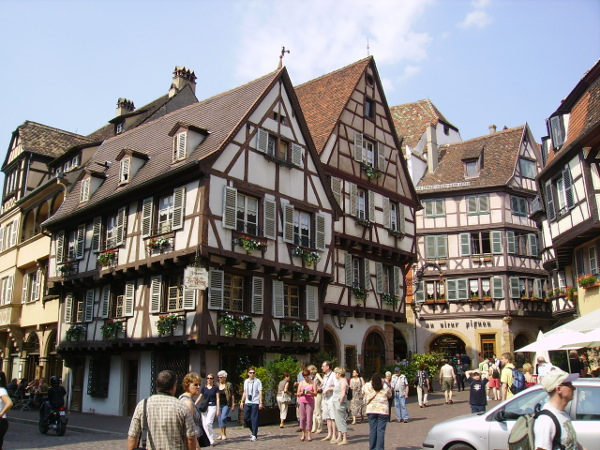
\includegraphics[scale=0.5]{images/architecturebretonne_wikipedia.jpg}
\caption{Éléments d'architecture bretonne typique du Sud de la France. (\href{http://commons.wikimedia.org/wiki/File:Colmar_-_Alsace.jpg}{Wikipédia.fr} CC-By-Sa)}
\end{figure}
\end{frame}
\end{comment}
\end{document}